\chapter{Results}
\label{chapter:results}

\section{\mbox{B-trees} and the choice of $b$}
At first, we fixed the $b$ parameter of \texttt{dict\_btree} to make nodes
exactly $64\,\text{B}$ in size to align them with physical cache lines.
This produces classic 2-3-4 trees. When we compared this \texttt{dict\_btree}
with simple red-black trees borrowed from LibUCW (\texttt{dict\_rbtree}),
we found them almost tied in performance (2-3-4 trees won by a small margin).

This was likely at least partially caused by the relatively small effective
branching factor of 2-3-4 trees (we measured 2.51 on $1\,000\,000$ random
keys).

\begin{figure}
\centering
\begin{subfigure}[t]{0.45\textwidth}
	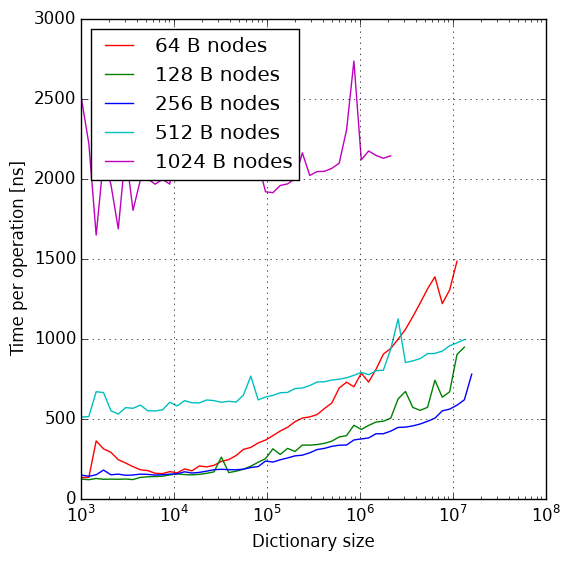
\includegraphics[width=\textwidth]{img/btree-b-find-50}
	\caption{Random \textsc{Find}s, 50\% successful (other success rates
		produce similar results)}
\end{subfigure}
~
\begin{subfigure}[t]{0.45\textwidth}
	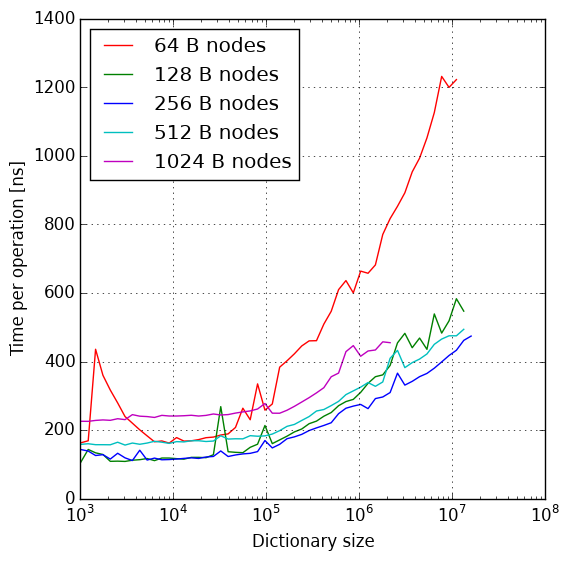
\includegraphics[width=\textwidth]{img/btree-b-insert}
	\caption{Random \textsc{Insert}s}
\end{subfigure}
\caption{The effect of different choices of $b$ on the performance of B-trees.
	Note that our initial choice ($64\,\text{B}$ nodes), performs
	particularly badly.}
\label{fig:btree-b-perf}
\end{figure}

We tried setting the size of nodes to larger powers of two, and we found
that nodes of $256\,\text{B}$ (i.e.,\ with 7--15 keys in internal nodes)
performed the best on random \textsc{Find}s and \textsc{Insert}s.
We used this node size in all of the following measurements.

Our code for B-trees uses linear search when looking within nodes.
With nodes this large, the speed of our code could possibly be improved
by using binary search.

\section{Basic cache-aware and unaware structures}
We compared our cache-aware B-trees trees to simpler, cache-unaware dictiories:
red-black trees borrowed from LibUCW and a simple sorted array with binary
search and $\O(N)$ updates. Note that a binary search needs
$\Theta(\log N-\log B)$ block transfers, which is asymptotically larger than
the $\Theta(\log_B N)$ required by B-trees.

\begin{figure}
\begin{subfigure}[t]{\textwidth}
	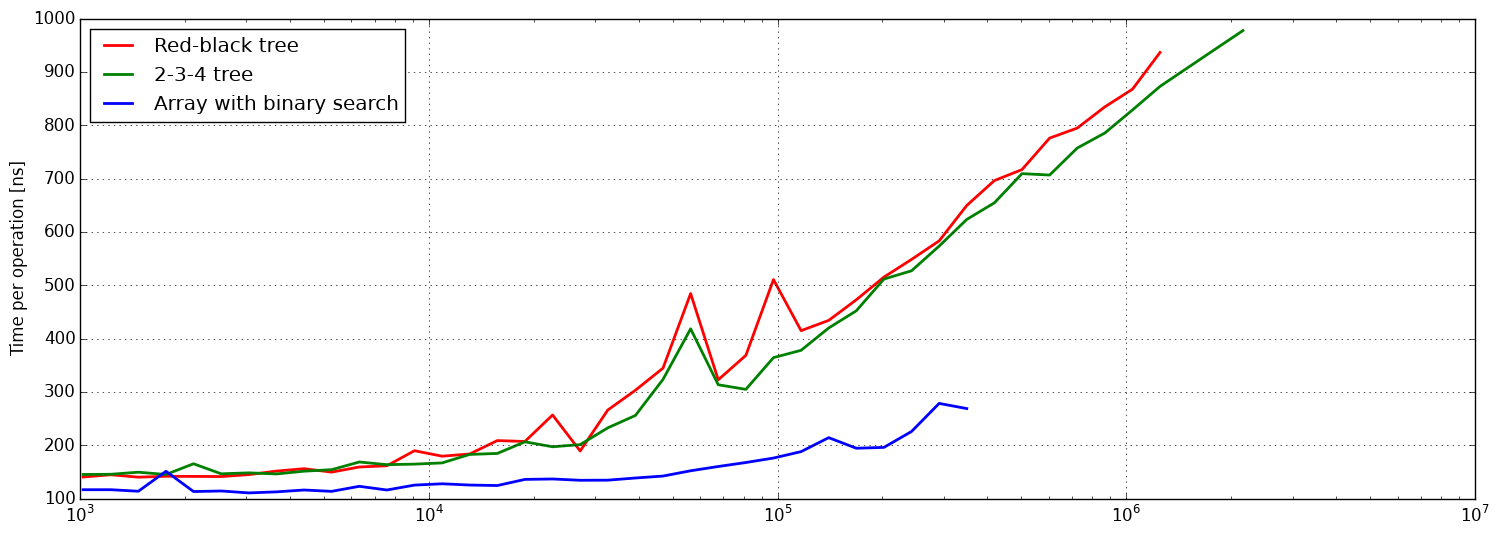
\includegraphics[width=\textwidth]{img/performance/basic-random-find-100}
	\caption{100\% success rate}
\end{subfigure}
\\
\begin{subfigure}[t]{\textwidth}
	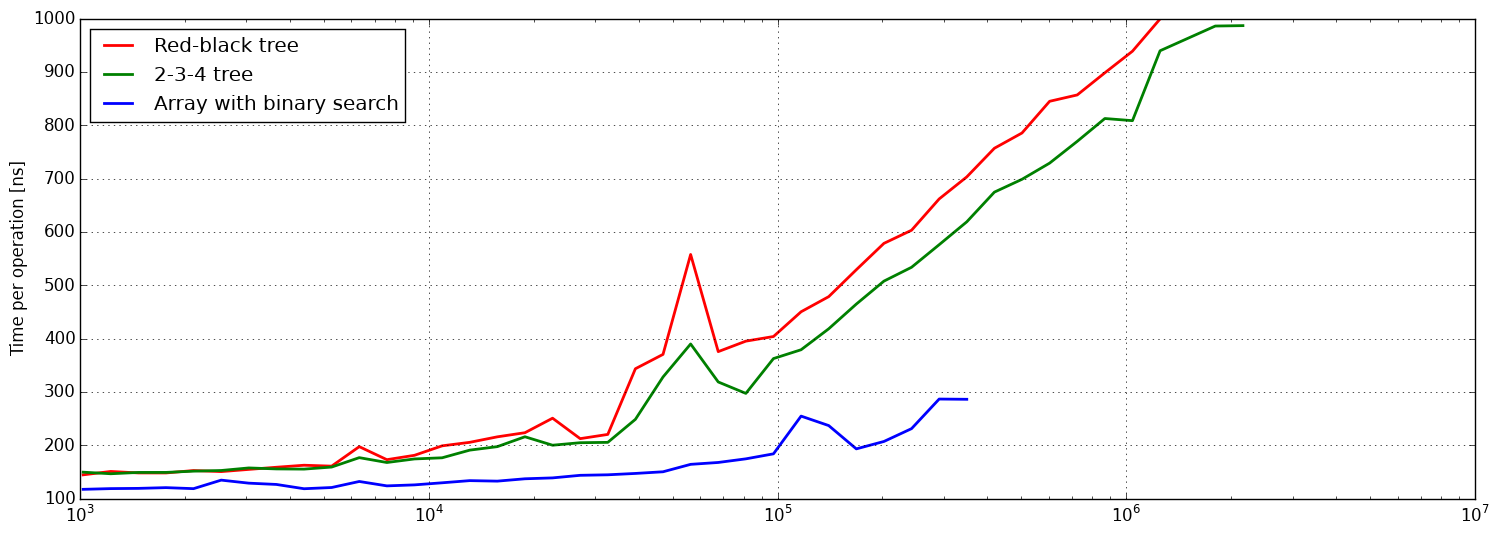
\includegraphics[width=\textwidth]{img/performance/basic-random-find-50}
	\caption{50\% success rate}
\end{subfigure}
\\
\begin{subfigure}[t]{\textwidth}
	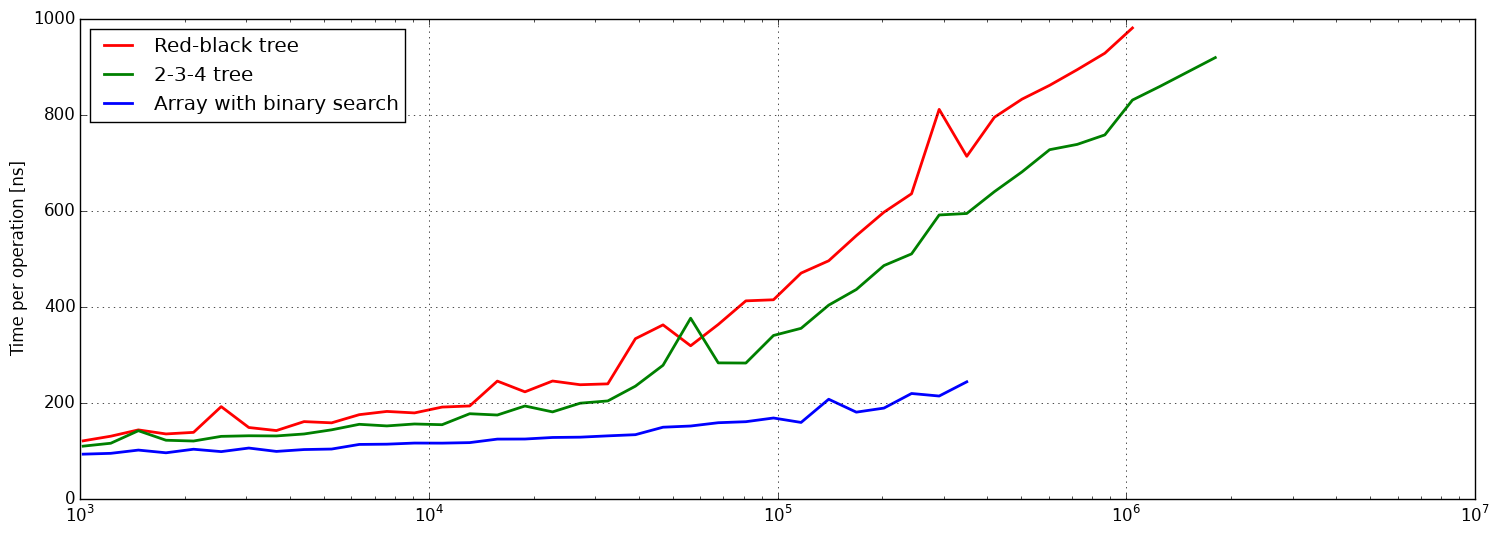
\includegraphics[width=\textwidth]{img/performance/basic-random-find-0}
	\caption{0\% success rate}
\end{subfigure}
\caption{Performance of random \textsc{Find}s in simple dictionaries.
	Arrays cut off early due to very slow insertions.}
\label{fig:basic-finds}
\end{figure}

\begin{figure}
\centering
\begin{subfigure}[t]{0.45\textwidth}
	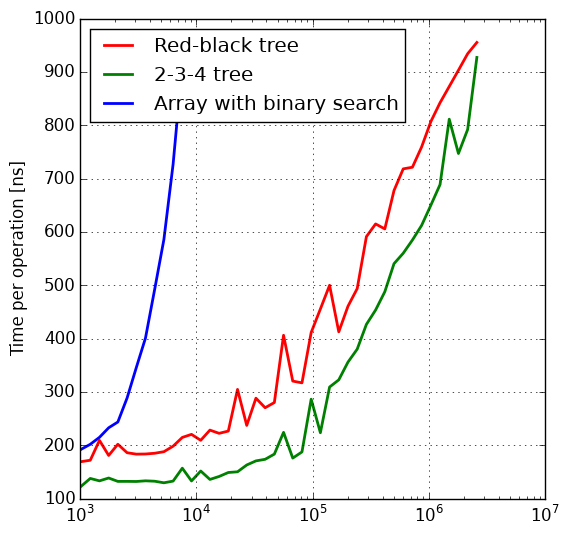
\includegraphics[width=\textwidth]{img/performance/basic-random-insert}
	\caption{Random \textsc{Insert}s}
\end{subfigure}
\caption{Performance of simple dictionaries. Arrays cut off early due to very
	slow insertions.}
\label{fig:basic-perf}
\end{figure}

Figures~\ref{fig:basic-finds} and \ref{fig:basic-perf} shows the results.
Red-black trees ended up slightly slower than our cache-aware B-trees.
We were slightly surprised that B-trees did not win over red-black
trees by a larger margin. The relatively small size of the difference

Interestingly, sorted arrays win on \textsc{Find}s, even if they are expected
to use more block transfers in the external memory model.

\section{Cache-oblivious B-tree}
\label{sec:cob-perf}
We found the performance of cache-oblivious B-trees very competitive compared
to B-trees on both random uniform access patterns and modestly large working
sets. As seen on figure~\ref{fig:cob-performance}, random successful
\textsc{Find}s were up to twice as fast in large cache-oblivious B-trees
without ever being significantly slower on small dictionaries.
The large density of the van Emde Boas tree is the likely reason for these
gains. In fact, the speeds of \textsc{Find}s in cache-oblivious B-trees
approached the speeds of \textsc{Find}s in arrays (compare
figure~\ref{fig:cob-performance} with figure~\ref{fig:basic-finds}).
\textsc{FindNext} and \textsc{FindPrev} are also faster in cache-oblivious
B-trees.

\textsc{Insert} operations, however, are comparatively slow in
smaller cache-oblivious B-trees (e.g.,\ $\leq$ 100~000 keys). We believe
this slowdown is probably due to the cost of rebuilds, which properly
amortizes away only on larger dictionaries. A~smarter choice of tuning
constants (i.e.,\ the minimum and maximum density and piece sizes) might
make updates of smaller dictionaries more efficient.

\begin{figure}
\centering
\begin{subfigure}[t]{0.45\textwidth}
	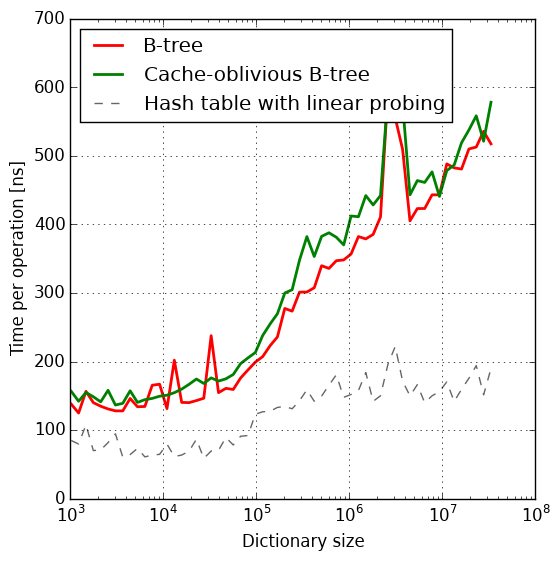
\includegraphics[width=\textwidth]{img/performance/cob-performance-1-100}
	\caption{Random \textsc{Find}s, 100\% successful (graphs for
		other success rates are very similar)}
\end{subfigure}
~
\begin{subfigure}[t]{0.45\textwidth}
	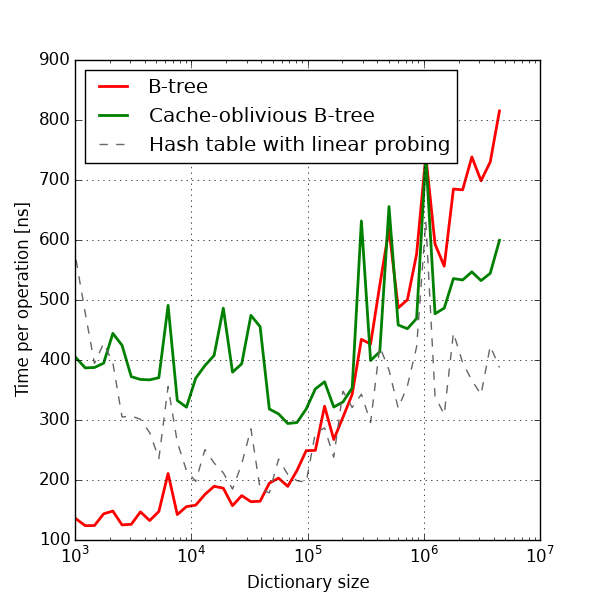
\includegraphics[width=\textwidth]{img/performance/cob-performance-2}
	\caption{Random \textsc{Insert}s}
\end{subfigure}
~
\begin{subfigure}[t]{0.45\textwidth}
	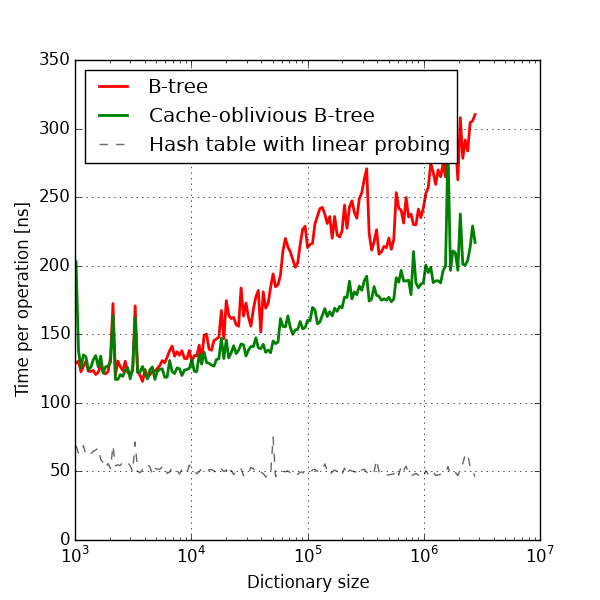
\includegraphics[width=\textwidth]{img/performance/cob-performance-3}
	\caption{Successful \textsc{Find}s, working set of 1~000 keys}
\end{subfigure}
~
\begin{subfigure}[t]{0.45\textwidth}
	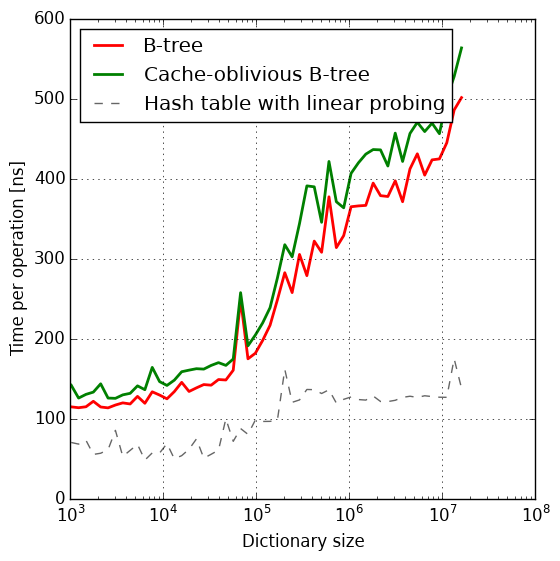
\includegraphics[width=\textwidth]{img/performance/cob-performance-4}
	\caption{Successful \textsc{Find}s, working set of 100~000 keys}
\end{subfigure}
~
\begin{subfigure}[t]{0.45\textwidth}
	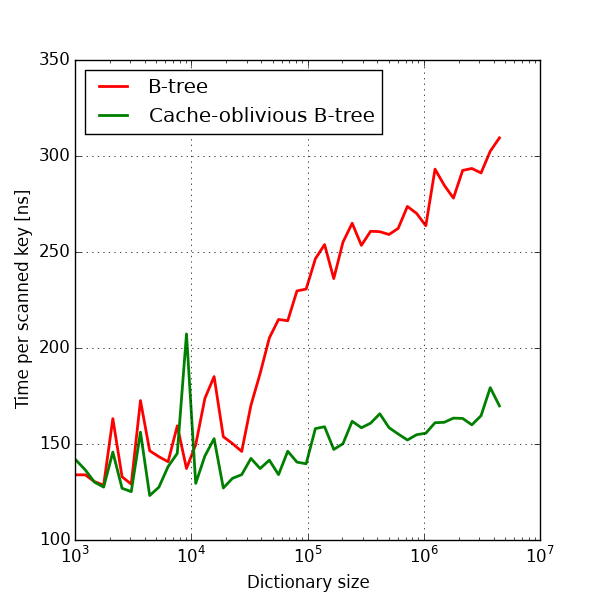
\includegraphics[width=\textwidth]{img/performance/cob-performance-5}
	\caption{Left-to-right scans over whole dictionary}
\end{subfigure}
~
\begin{subfigure}[t]{0.45\textwidth}
	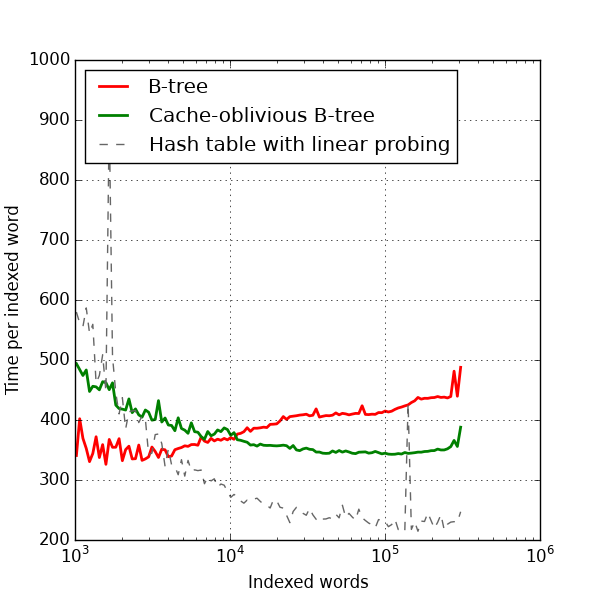
\includegraphics[width=\textwidth]{img/performance/cob-performance-6}
	\caption{Word occurrence counting}
\end{subfigure}
\caption{Benchmarks of cache-oblivious B-trees.
	Measurements of hash table with linear probing included for reference.}
\label{fig:cob-performance}
\end{figure}

\section{Self-adjusting structures}
Splay trees are the canonical self-adjusting structure we would like to
outperfrom. As expected, splay trees are somewhat slower than B-trees on
unpredictable operations (see figure~\ref{fig:self-adj-performance-finds}).

\begin{figure}
\begin{subfigure}[t]{\textwidth}
	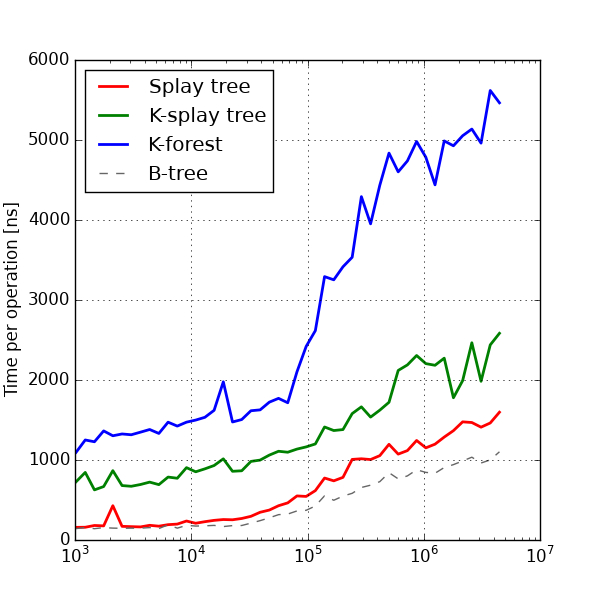
\includegraphics[width=\textwidth]{img/performance/self-adj-random-find-100}
	\caption{100\% success rate}
\end{subfigure}
\\
\begin{subfigure}[t]{\textwidth}
	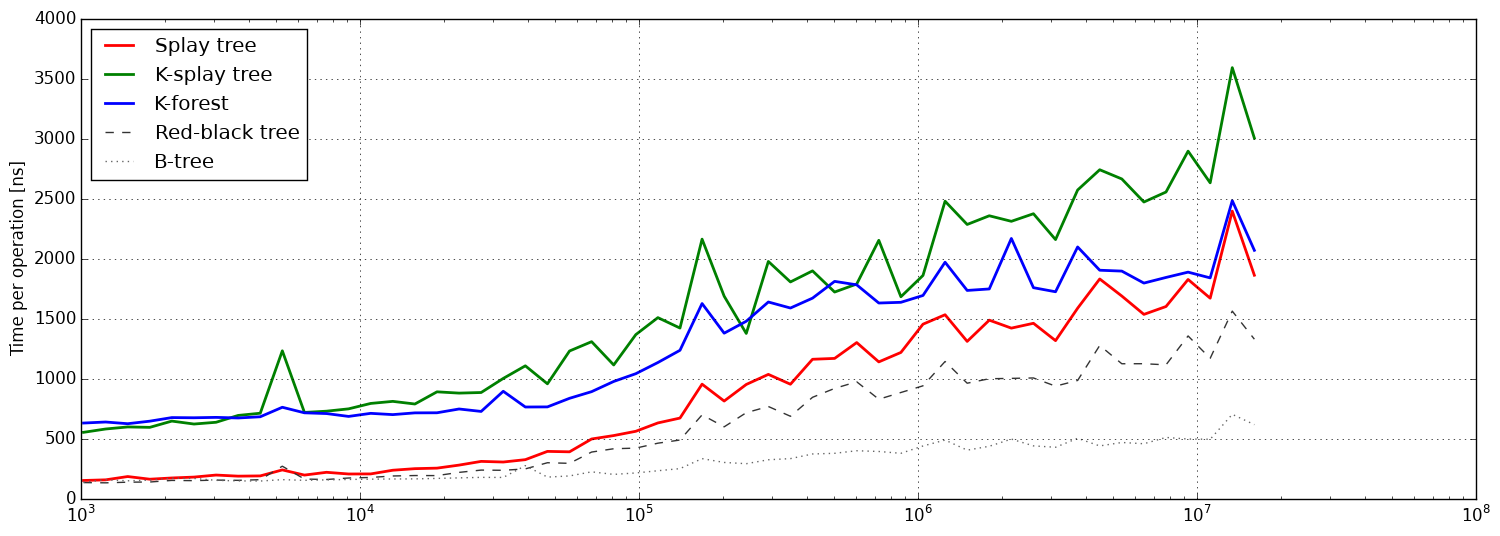
\includegraphics[width=\textwidth]{img/performance/self-adj-random-find-50}
	\caption{50\% success rate}
\end{subfigure}
\\
\begin{subfigure}[t]{\textwidth}
	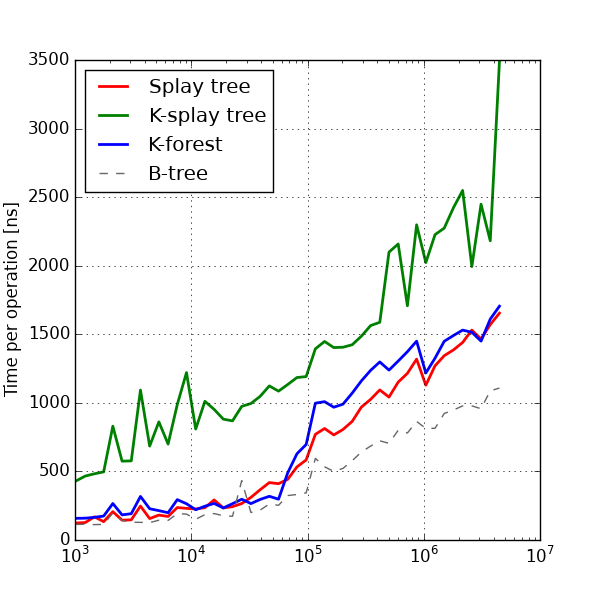
\includegraphics[width=\textwidth]{img/performance/self-adj-random-find-0}
	\caption{0\% success rate}
\end{subfigure}
\caption{Performance of random \textsc{Find}s in self-adjusting structures}
\label{fig:self-adj-performance-finds}
\end{figure}

\begin{figure}
\begin{subfigure}[t]{0.31\textwidth}
	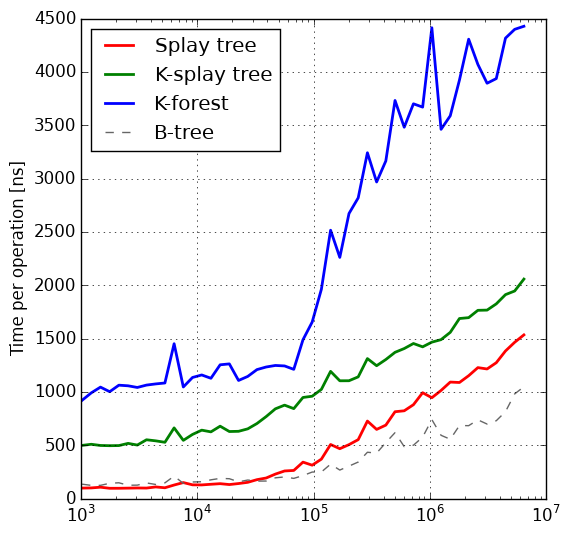
\includegraphics[width=\textwidth]{img/performance/self-adj-random-insert}
	\caption{Random \textsc{Insert}s}
\end{subfigure}
~
\begin{subfigure}[t]{0.31\textwidth}
	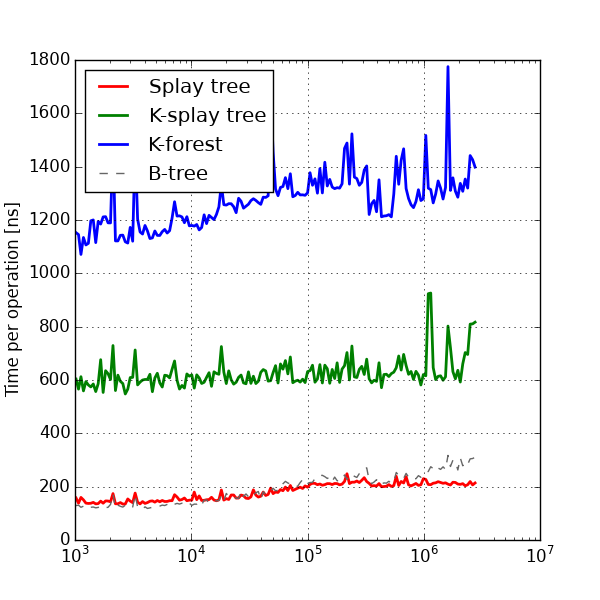
\includegraphics[width=\textwidth]{img/performance/self-adj-ws-1k}
	\caption{Successful \textsc{Find}s, working set of 1~000 keys}
	\label{fig:sub:self-adj-ws-1k}
\end{subfigure}
~
\begin{subfigure}[t]{0.31\textwidth}
	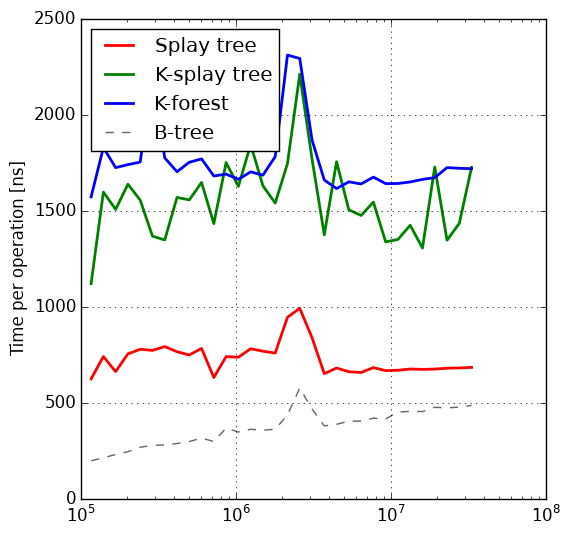
\includegraphics[width=\textwidth]{img/performance/self-adj-ws-100k}
	\caption{Successful \textsc{Find}s, working set of 100~000 keys}
	\label{fig:sub:self-adj-ws-100k}
\end{subfigure}
% TODO: word occurrence counting
\caption{Benchmarks of self-adjusting structures.
	B-trees are included for reference.}
\label{fig:self-adj-performance}
\end{figure}

Unfortunately, we found both $k$-splay trees and $k$-forest lacking in
performance in every experiment.

Profiling our performance tests running on $k$-splay trees showed that about
21\% of time is spent in \texttt{ksplay\_walk\_to}, which finds the correct
leaf for a key and puts the path to the leaf into a buffer. About 37\% of the
time is taken by \texttt{ksplay\_step}, which performs a splaying step, along
with helper functions it calls (\texttt{flatten\_explore},
\texttt{compose\_twolevel}).

One suboptimal property of our implementation is that it dynamically
allocates the $k$-splayed path on every $k$-splay. Memory allocation alone
accounts for about 20\% of CPU time.
We experimented with replacing memory allocation with a static array.
This change brought the performance of $k$-splay trees somewhat closer to
splay trees, but splay trees still won in every test
(see figure~\ref{fig:ksplay-noalloc}).

\begin{figure}
\begin{subfigure}[t]{0.48\textwidth}
	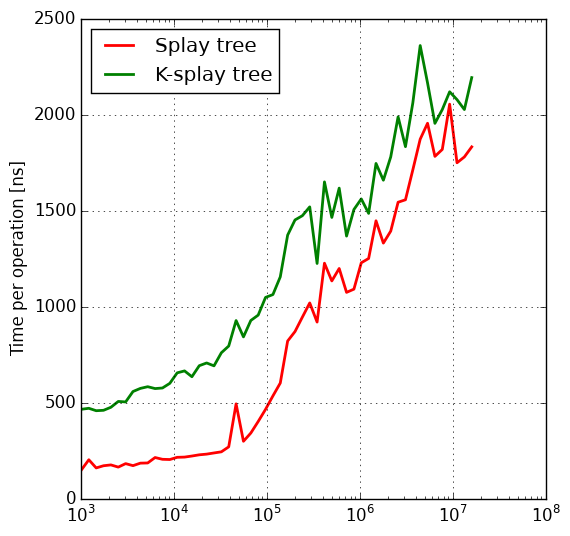
\includegraphics[width=\textwidth]{img/ksplay-noalloc-find-50}
	\caption{Random \textsc{Find}s, 50\% success rate}
\end{subfigure}
~
\begin{subfigure}[t]{0.48\textwidth}
	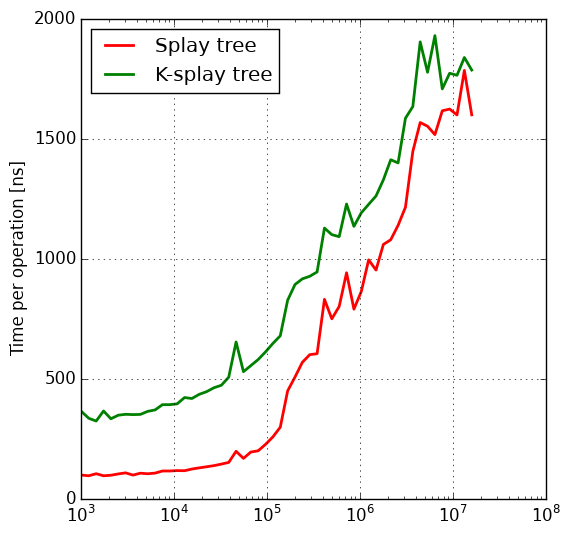
\includegraphics[width=\textwidth]{img/ksplay-noalloc-insert}
	\caption{Random \textsc{Insert}s}
\end{subfigure}
\caption{The performance of $k$-splay trees with removed temporary heap
	allocation, compared to splay trees}
\label{fig:ksplay-noalloc}
\end{figure}

As suggested in \cite{ksplay-sherk}, it should be possible to remove the
need to store the splayed path by top-down \mbox{$k$-splaying}.
Unfortunately, even top-down \mbox{$k$-splaying} needs to touch
$\Theta(k^2)$ keys and pointers in every $k$-splay step, so we believe top-down
\mbox{$k$-splaying} would not significantly reduce the high cost of
\texttt{ksplay\_step}.

Our measurements on small working sets
(figure~\ref{fig:self-adj-performance}\subref{fig:sub:self-adj-ws-1k},
\subref{fig:sub:self-adj-ws-100k}) confirm that splay trees, $k$-forests
and $k$-splay trees all have the working set property.
Even if we only use a small working set, B-trees need more data to reach
the sought key-value pairs as we increase the size of the dictionary, because
values are stored in leaves, which are lower in bigger B-trees.
Unlike B-trees, splay trees and $k$-splay trees can keep the small working set
close to the root, even as we add many unused key-value pairs into the
dictionary.

Due to the presence of caches, even non-self-adjusting data structures (like
\mbox{B-trees}) can exhibit a ``pseudo-working set property'', provided
the auxiliary data needed to access the working set fits into the cache.
However, as we increase the size of the dictionary, we can distinguish
the ``pseudo-working set property'' from the true working set property:
in B-trees, more auxiliary data is needed, and it eventually ceases to fit
in the cache.
In structures with the true working set property, caches will still contain
mostly useful key-value pairs, even when the working set is a tiny fraction
of the dictionary.

$k$-forests were slow both backed by B-trees and by cache-oblivious B-trees.
Choosing a larger $k$ slightly helped, but larger values of $k$ also degenerate
\mbox{$k$-forests} into their backing structure.
As observed on figure~\ref{fig:self-adj-performance-finds}, \textsc{Find}s in
$k$-forests are much slower when they are successful, probably due to the need
to promote the found key-value pair. A possible way of speeding up
\textsc{Find}s may be backing the \mbox{$k$-forest} by a structure that can
support fast promotions and demotions without complicated structural changes.

\section{Hashing}
\label{sec:hashing-results}
We compared a hash table with linear probing to a cuckoo hash table.
Both hash tables used a bytewise simple tabulation hash function.
The cuckoo hash table maintained a load factor between $1/4$ and
$1/2$ and the hash table with linear probing had a load factor
between $1/4$ and $3/4$.

Since cuckoo hash tables guarantee worst-case $\O(1)$ time for lookups,
we expected both successful and unsuccessful random \textsc{Find}s to be
measurably slower with linear probing.
On random successful \textsc{Find}s (figure~\ref{fig:hashing-performance-finds}\subref{fig:sub:hashing-1-100}),
cuckoo hashing did only very slightly better than linear probing.
On unsuccessful \textsc{Find}s (figure~\ref{fig:hashing-performance-finds}\subref{fig:sub:hashing-1-0}),
the benefits of cuckoo hashing were more pronounced.
On the other hand, linear probing allows a higher load factor.
(Forcing cuckoo hashing to fill the hash tables more fully significantly
slows down \textsc{Insert}s.)

\textsc{Insert}s into cuckoo hash tables proved significantly slower.
One possible reason might be the limited independence guaranteed by simple
tabulation hashing.

\begin{figure}
\begin{subfigure}[t]{\textwidth}
	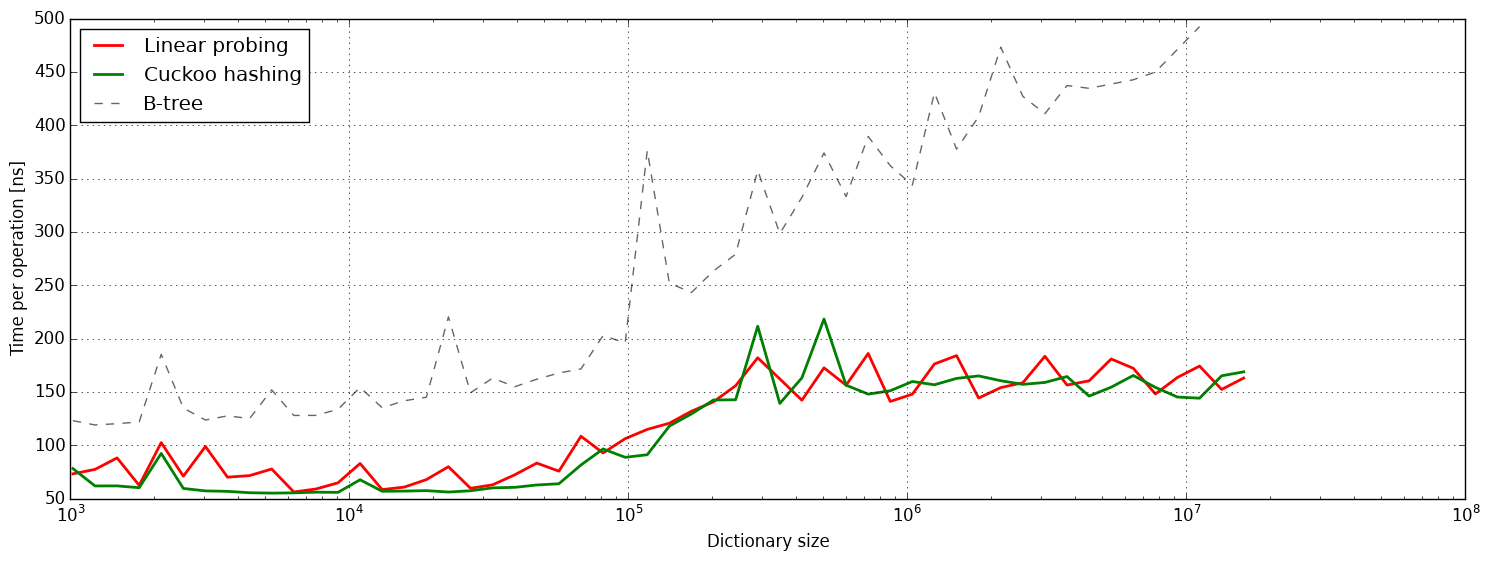
\includegraphics[width=\textwidth]{img/performance/hashing-1-100}
	\caption{100\% success rate}
	\label{fig:sub:hashing-1-100}
\end{subfigure}
\\
\begin{subfigure}[t]{\textwidth}
	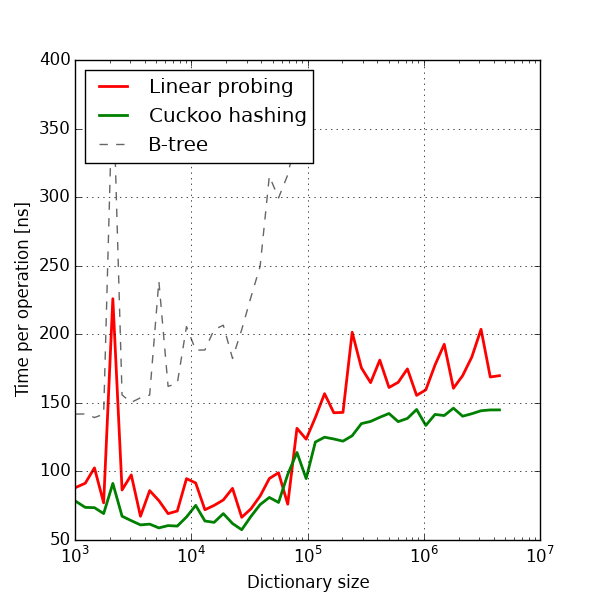
\includegraphics[width=\textwidth]{img/performance/hashing-1-50}
	\caption{50\% success rate}
\end{subfigure}
\\
\begin{subfigure}[t]{\textwidth}
	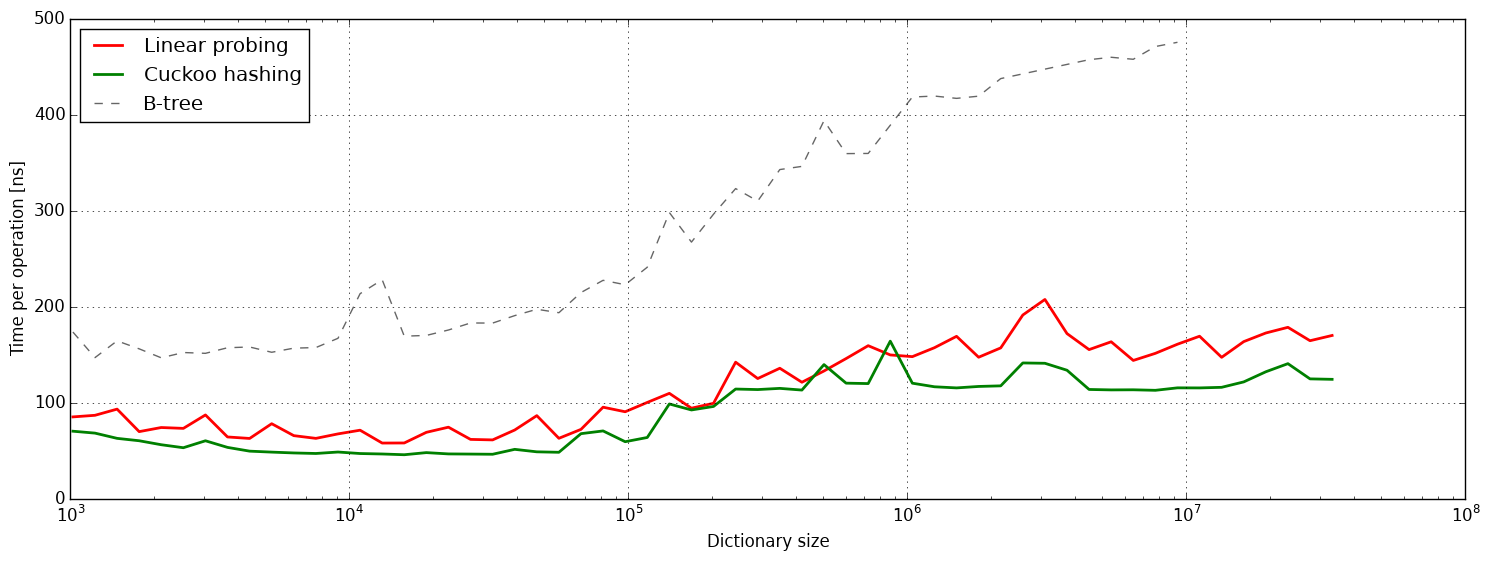
\includegraphics[width=\textwidth]{img/performance/hashing-1-0}
	\caption{0\% success rate}
	\label{fig:sub:hashing-1-0}
\end{subfigure}
\caption{Performance of random \textsc{Find}s in cuckoo hashing and linear probing}
\label{fig:hashing-performance-finds}
\end{figure}

\begin{figure}
\begin{subfigure}[t]{0.31\textwidth}
	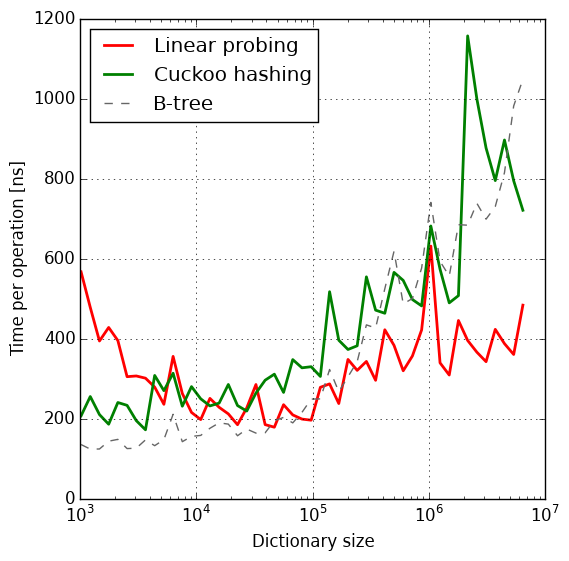
\includegraphics[width=\textwidth]{img/performance/hashing-2}
	\caption{Random \textsc{Insert}s}
\end{subfigure}
~
\begin{subfigure}[t]{0.31\textwidth}
	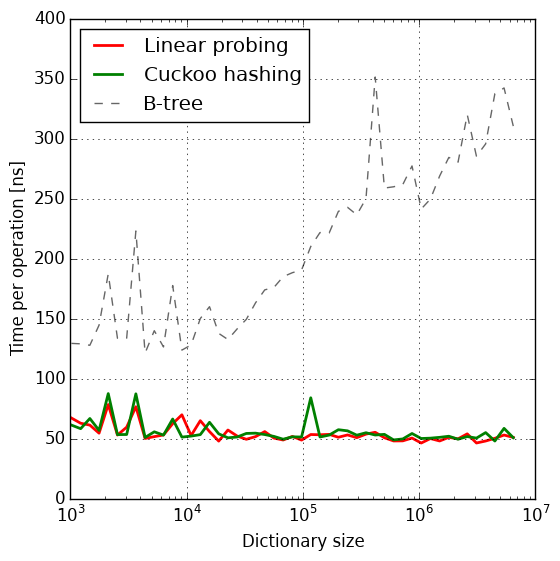
\includegraphics[width=\textwidth]{img/performance/hashing-3}
	\caption{Successful \textsc{Find}s, working set of 1~000 keys}
\end{subfigure}
~
\begin{subfigure}[t]{0.31\textwidth}
	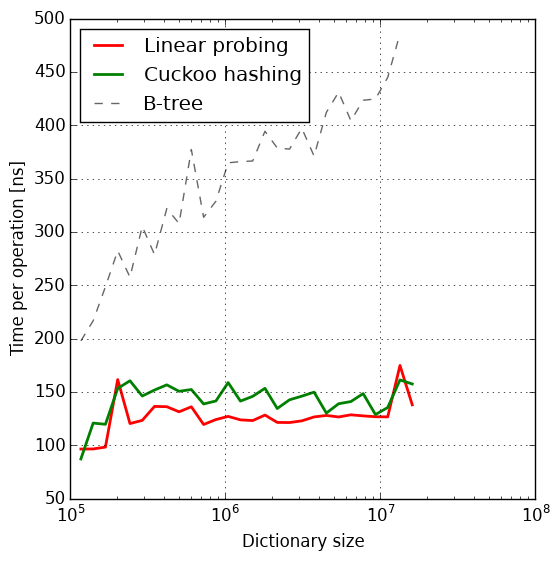
\includegraphics[width=\textwidth]{img/performance/hashing-4}
	\caption{Successful \textsc{Find}s, working set of 100~000 keys}
\end{subfigure}
\caption{Performance of cuckoo hashing and linear probing on \textsc{Insert}s
	and \textsc{Find}s in working sets}
\label{fig:hashing-performance}
\end{figure}

\section{Practical experiments}
\subsection{Mozilla Firefox}
The hash table operations collected from the Firefox session are compressed
in \texttt{data/firefox-htable.tar.gz}. We replayed the operations on all our
dictionary implementations. We normalized the measured times by the maximum
time taken for each recording to allow easier comparison of relative
performance. Our results are presented in table~\ref{tab:firefox-results}.

%\begin{table}
\begin{sidewaystable}
\centering
% TODO: Sort!
\begin{tabular}{|c|r|r|r|r|r|r|r|r|r|}
	\hline
	Recording &
		Array & Red-black tree &
		B-trees & COBT &
		Splay & $k$-forest & $k$-splay &
		Linear probing & Cuckoo \\

	\hline
	\texttt{0x7f47930300e0} & 14 & 16 & 15 & 13 & 14 & 100 & 91 & 6 & \textbf{4} \\
	\hline
	\texttt{0x7f566e3cb0e0} & 10 & 7 & 8 & 10 & 11 & 100 & 78 & 9 & \textbf{6} \\
	\hline
	\texttt{0x7fff84eb8f98} & 13 & 11 & 12 & 14 & 13 & 64 & 100 & 11 & \textbf{6} \\
	\hline
	\texttt{0x7fff1d9c7738} & 16 & 16 & 15 & 15 & 14 & 58 & 100 & 14 & \textbf{6} \\
	\hline
	\texttt{0x7fff84eb9148} & 14 & 11 & 12 & 14 & 12 & 70 & 100 & 12 & \textbf{7} \\
	\hline
	\texttt{0x7f567b64a830} & 100 & 8 & 7 & 6 & \textbf{1} & 42 & 30 & 4 & 4 \\
	\hline
	\texttt{0x7f4791631c60} & 11 & 12 & 11 & 17 & \textbf{9} & 34 & 100 & 15 & 13 \\
	\hline
	\texttt{0x7f5671faab80} & 20 & 15 & 18 & 28 & \textbf{11} & 18 & 100 & 24 & 22 \\
	\hline
	\texttt{0x7f47a6e31058} & 10 & \textbf{7} & 11 & 15 & 10 & 13 & 100 & 16 & 19 \\
	\hline
	\texttt{0x7f565ca63148} & 8 & \textbf{8} & 9 & 12 & 12 & 46 & 100 & 13 & 10 \\
	\hline
	\hline
	Average & 22 & 11 & 12 & 14 & 11 & 55 & 89 & 12 & 10 \\
	\hline
\end{tabular}
\caption{Results of the Mozilla Firefox experiment. Standardized by maximum
	time (lower is better). Sorted by which implementation is fastest.
	Produced by \texttt{experiments/vcr/make\_table.py}.}
\label{tab:firefox-results}
%\end{table}
\end{sidewaystable}

Overall, the cache-oblivious B-tree (COBT) performed slightly worse than
\mbox{B-trees} in this experiment. We believe this may be explained by the
small size of typical hash tables, which forces frequent costly rebuilds of
the packed memory array.

Interestingly, red-black trees outperformed cache-aware B-trees
on the Firefox recordings even through our synthetic experiments ran slightly
faster on B-trees.
One possible explanation is the presence of \textsc{Delete}s in the recording --
we did not perform any experiment to explicitly measure their speed.

Most recordings run fastest either on cuckoo hash tables, or on splay trees.
By inspecting the recordings, we found that splay trees are better on recordings
with many updates, while cuckoo tables win when there are much more
\textsc{Find}s. Choosing the wrong structure can reduce the performance,
typically about $2\times$, but, as seen in the case of \texttt{0x7f47930300e0},
the difference can be up to $4\times$.
We believe a data structure that would dynamically switch
its internal representation between cuckoo hashing and splay trees
based on the access pattern may be a~good compromise.

Interestingly, linear probing does not behave as well on Firefox recordings
as in synthetic experiments, in which it performed as well as cuckoo hashing
in random \textsc{Find}s and slightly better on \textsc{Insert}s. One possible
reason for this is a higher incidence of failed \textsc{Insert} and
\textsc{Find} operations. As we observed above, failed \textsc{Find}s are
faster with cuckoo hashing, as they take only 2 memory transfers as any other
\textsc{Find}, while an unsuccessful \textsc{Find} with linear probing needs to
traverse an entire chain.

\subsection{Geospatial database}
The results of the cloud database experiment are outlined in
table~\ref{tab:cloud-results}. Cache-oblivious \mbox{B-trees} slightly outperformed
standard \mbox{B-trees}. Splay trees were surprisingly fast. One factor that
might cause them to perform so well might be that stations usually produce
a~large amount of reports over their lifetime, so when we fetch $S$ closest
reports for a~point, it is likely that all such reports will be the first $S$
reports reported by the closest station. Splay trees may thus keep old reports
near the top. In this experiment, we picked $S=1~000$. Also, as can be
seen on figure~\ref{fig:cloud-data}, the distribution of stations on the globe
is very uneven, so stations ``assigned'' to a large area can be kept closer to
the root.

Additionally, we tried two algorithms for sampling query points on the globe.
The first algorithm simply iterated through points on the latitude-longitude
grid with whole number coordinates (i.e.,\
$179.0\degree\,\text{W}\ 90.0\degree\,\text{N}$ through
$180.0\degree\,\text{E}\ 90.0\degree\,\text{S}$).
The second algorithm arbitrarily picked $64~800=180\cdot 360$ random query
points.
The algorithm can be selected by passing different values of the
\texttt{--scatter} flag to the \texttt{bin/experiments/cloud} binary
(\texttt{--scatter=GRID} for grid sampling, or \texttt{--scatter=RANDOM
--samples=64800} for random sampling).

All data structures performed slightly better on the first one, which shows
that more predictable accesses are better for performance. The effect was,
however, comparatively weak on cache-oblivious B-trees.

\begin{table}
\centering
\begin{tabular}{|c|S<{\,\si{\s}}|S<{\,\si{\s}}|}
% TODO: add dict_rbtree
%--close_count=1000
%--scatter=GRID
%--lat_step=100
%--lon_step=100
%--min_year=1997
%--max_year=2005 ===>
%	       dict_cobt:     20 687 539 351 ns
%	      dict_splay:      6 030 131 877 ns
%	     dict_ksplay:     41 687 825 004 ns
%	      dict_btree:     22 677 805 459 ns
%
%--samples=64800 (180*360)
%--scatter=RANDOM ===>
%	       dict_cobt:     20 583 667 067 ns
%	      dict_splay:      6 647 207 153 ns
%	     dict_ksplay:     44 717 377 069 ns
%	      dict_btree:     25 884 347 926 ns
	\hline
	Dictionary & \multicolumn{1}{c|}{Grid sampling} & \multicolumn{1}{c|}{Random sampling} \cr
	\hline
	Cache-oblivious B-tree & 20.69 & 20.58 \cr
	\hline
	Splay tree & 6.03 & 6.65 \cr
	\hline
	$k$-splay tree & 41.69 & 44.72 \cr
	\hline
	B-tree & 22.68 & 25.89 \cr
	\hline
\end{tabular}
\caption{Results of the cloud database experiment, generated
	by \texttt{bin/experiments/cloud --max\_year=2005}.
}
\label{tab:cloud-results}
\end{table}
